\documentclass[10pt]{article}

\usepackage{textcomp} % use \textmu to add micro symbol
\usepackage[english]{babel}

\usepackage{fancyhdr} % only header on fancy pages
\fancyhf{}
\fancyhead[C]{CS472 D. Kevin McGrath}

\usepackage{sectsty} % modify section header style
\sectionfont{\fontsize{14}{21}\selectfont}
\makeatletter
\def\@seccntformat#1{\protect\makebox[0pt][r]{\csname
                     the#1\endcsname\quad}}
\makeatother

\nocite{*}

\usepackage{graphicx}
\graphicspath{ {./images/} }

\setlength{\parindent}{3em}
\setlength{\parskip}{3pt}
\renewcommand{\baselinestretch}{1.1}

\title{Comparison of PowerPC Architecture \& Intel x86} 
\author{Neale Ratzlaff}

\begin{document}
\maketitle
\thispagestyle{fancy} % first page is fancy

\section{History of PowerPC and IA}

\textsc{In} 1991, IBM, in tandem with its partners Apple and Motorola developed their Performance Optimization With Enhanced RISC – Performance Computing machine (PowerPC). The PowerPC (PPC) was developed as a RISC computing system for personal use, built on top of the POWER ISA that was developed by IBM in 1990. The system found its use in Apple`s original machines before the switch to IA as one popular implementation of the system. The PowerPC featured a fused multiply-add, little and big endian support, double precision floating point operations, and a paging memory architecture, among other features that will be discussed later.  In 1991 IBM approached Apple with the prospect of a joint project that would yield a processor family based on the POWER ISA. Motorola joined the table when approached by Apple with the same goal. At that time, most computers were driven by Intel 80386 processors, and RISC was poorly represented in PCs. When the PowerPC hit the market later that year it did quite well, with Microsoft and Sun Microsystems developing Windows NT 3.51 and a compatible Solaris OS respectively for the PPC. Through the 1990s the PPC was benchmarked at and above the top x86 processors. But the opportunity for a desktop class architecture never came to fruition. Only Apple kept the PPC alive by insisting on the PPC’s presence in its machines.  Then in 2004, IBM sold the PowerPC line to AMCC, and Motorola moved its semiconductor business completely over to Freescale Semiconductor. Apple moved to Intel CPUs in 2005, citing worries over efficiency and power consumption of the PowerPC. Today IBM continues to develop the PowerPC architecture as cores in the ASIC design market. PowerPC and POWER have merged back into the POWER architecture, and is managed jointly by IBM, Freescale, and AMCC
\par
x86 however, is much older, first released in 1978 on the Intel 8086 CPU as a CISC architecture. It was a 16 bit processor that featured fourteen 16-bit registers. It had four general purpose registers, two special registers: a stack pointer and a base pointer, four segment registers to form a memory address, and a flag register for status. The 8086 gained popularity for its ability to translate assembly programs written for the 8080 into compatible programs, as well as IBM’s decision to put the 8088 into their IBM PC. The next advance was in making the 32 bit 8086 compatible 80386. Intel focused on the 8086 line after the market failure of the 32 bit 8800. i483 was the first fully pipelined x86 processor which set the stage for the Pentium family. The architecture has continued to improve each year, driving many of the important architectural advances seen in modern processors. x86 offers many features which have become standard, such as Multimedia Extensions (MMX), Streaming SIMD Extensions (SSE), Physical Address Extensions (PAE), and many others. x86 now describes almost all of Intel`s processors. The popular Intel Core line of processors was released in 2006 with the Celeron. It featured 3 levels of cache and dual cores. The Core architecture continues today with the Core i3, i5, and i7. The Intel Xeon line, a family of processors aimed at server infrastructure is the main non-consumer product line offered by Intel. The Xeons feature many more cores than a Core processor up to 18 cores in the Xeon E7 family. The cores, though numerous, are typically low clock speed of 1 - 2 GHz. Low clock speeds make more sense for a multicore server system. The expected loads are not large enough to warrant a super-fast core, many parallel units will offer the lowest latency and largest throughput. There is one tier above the Xeons that is not in fact x86. The Xeon Phi family is build upon Intel`s Many Integrated Core (MIC) architecture, and offers server solutions of 72 core boards. MIC offers some crossover instructions from x86, but does not include MMX, SSE, or AVX compatibility. The speed increase in so many cores comes from parallelization and vectorization, so it may not be useful to have these parts of the x86 ISA at all.  
\par

\section{Instruction Set}

\textsc{The} PowerPC ISA is extremely RISC-like, with most instructions taking only one cycle to decode. The ISA can take advantage of 32 general purpose registers (GPRs), 32 floating point registers (FPRs), and various other control registers. All PPC instructions are single-word 32 bit instructions, this simplifies the pipelining process greatly, the PPC does not need the die space IA needs to fit in their CISC decoding circuitry. The ISA features integer instructions, floating point instructions, load-store instructions, synchronization instructions, flow control, and memory/cache control instructions.  The integer and floating point instructions are indicative of the PPCs RISC nature, as they are all single cycle instructions like compare, fused multiply-add, and logical operations. The load/store operations are special to the load/store unit and can load/store string instructions, multiple arithmetic instructions, or byte reverse instructions for endianness flipping. Synchronization instructions are mainly utilized in the context of the load/store unit. These instructions allow the processor to process IO operations out of order, or to load/store operations on a bus that is shared by multiple devices. Flow control instructions are standard branching and trap instructions. Finally the memory management instructions allow fine grain control over the L1 and L2 cache, TLBs, and segment registers used for address translation.  
\par
IA by contrast has an intense instruction set that consists of hundreds of instructions. Because IA is CISC at heart, it doesn’t have to break down instructions into primitives. CISC instructions do the equivalent of multiple RISC instructions. IA instructions take advantage of the huge amount of extensions that come with Intel processors. MMX and SSE instructions are among the many instructions that IA includes, that don`t have a one to one counterpart in PPC. 
\par

\section{Data Path and Pipeline}

\textsc{The} PPC has been pipelined since the introduction of the PPC 601. After development into the 900 series the pipeline expanded from 3 stages into the standard 5 areas: fetch, decode, execute, access, writeback. The PPC 750 had a four stage pipeline for integer instructions, however it only has the ability to complete two instructions per cycle. The PPC 750 also features a branch prediction unit called a Branch Table (BT), similar to x86. The BT can predict on four branches in parallel, and uses Yeh`s algorithm to determine if the branch is to be taken or not based on previous branches taken. Yeh`s algorithm is a two stage adaptive predictor, which essentially can quickly learn local branch patterns with an accuracy of ~97\% . The BT also has the capacity to look two branches deep, and store the first two instructions held there. If a branch is predicted to be taken, then these instructions are popped off the stack and loaded. In this way, PPC can achieve a zero cycle branch. 
\par
All PowerPC instructions are decoded in a single cycle, showing the RISC nature of the architecture. The decoded instructions are then held in a reorder buffer who will commit the instructions in program order. The PPC has eight execution units in the 750, and can retire up to two instructions per cycle. In order to be retired by the completion unit (CU) the instruction must have been executed correctly with no missed branches and was next in program order 
\par
\begin{figure}[h]
   \centering
   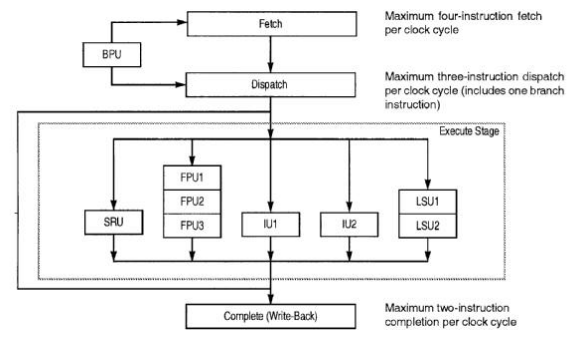
\includegraphics[scale=0.5]{PPC_pipeline}
   \caption{PowerPC 4 Stage Pipeline}
\end{figure}
\par
In the case of pipelining hazards, PPC needs to retain a sequential execution model. Data hazards can occur after improper IO. This is a natural consequence of out of order (OOO) execution in the pipeline, Instructions may rely on the output of another instruction, but OOO execution may cause the dependant instruction to be executed earlier than its parent. PPC handles a data hazard in many cases by stalling the dependant instruction until the parent can be processed, and the necessary operand made available. Register names may also be renamed, using shadow registers that share the same data as their counterpart. By dynamically renaming registers, instructions that reach into the same register may be segmented into multiple parallel units. 
\par
Control Hazards also handled with stalling, the related instruction is blocked until the branch in question is resolved. This approach is often  abandoned in favor of branch prediction which is used if successful, otherwise the system defaults to blocking. Branches are predicted by storing the target addresses of all branches taken in the past by the program. If the target address is requested again by a branch instruction, the address will be loaded from the Branch Target Address Cache (BTAC) if the branch confidence is strong. Structural Hazards are handled by duplicating resources need by the competing instructions. 
\par
\begin{figure}[h]
   \centering
   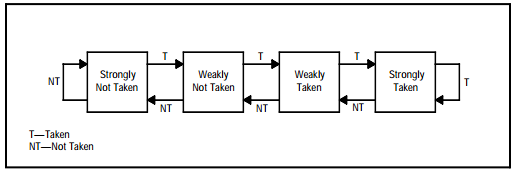
\includegraphics[scale=0.5]{PPC_branch}
   \caption{Yeh's Branch Prediction Algorithm (2 bit)}
\end{figure}
\par
The Intel pipeline has historically been much more varied than PPC. The original 8086 had no pipeline at all, instead it fetched, decoded, and executed all instructions sequentially from a queue. The current Intel Core pipeline is 14 stages long. The actual format of the IA pipeline is similar to PPC’s, in that they both can be broken down into the basic five stage pipeline. The capabilities with respect to the stages of the pipeline differ, however. Core has a four-wide decode unit, allowing the unit to decode up to four separate instructions per cycle, or five if the processor is in Macrofusion mode. Macrofusion is one of the features present in IA that has no analog in the PPC. Macrofusion takes two common instructions that have a known outcome, and fuses them into a single instruction. This is done at the decoder and retirement unit to increase throughput. Once the instructions are broken down into micro-ops, the pipeline can retire up to four micro-ops per cycle. This is two more than the PPC, and because IA is CISC-like, the computational ability of retiring four instructions is likely more than double the throughput of retiring two RISC instructions in a cycle.  IA also offers full branch prediction using Branch Target Buffers (BTB) by representing branches as objects called traces. Traces are stored in the trace cache, and are analysed for the most likely branch to be taken. In this way, branches that are predicted to be taken are loaded for a zero cycle branch overhead as the prefetched branch becomes the new instruction source. When micro-ops are completed, the retirement unit commits the results in program order, and updates the BTBs with past branches taken, as with the PPC. 
\par
\begin{figure}[h]
   \centering
   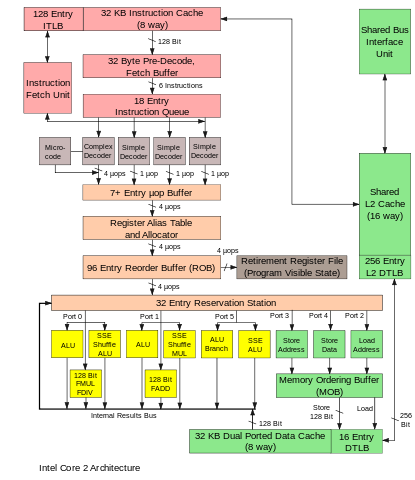
\includegraphics[scale=0.5]{IA_pipeline}
   \caption{x86 Core 2 Pipeline}
\end{figure}
\par

\section{Memory Heirarchy}

\textsc{The} PPC 750 shipped with a 64KB L1 cache, with 32KB each for instruction and data. The L1 is 32B line size, eight-way set associative. There was also the option for an two-way associative, 1024KB, unified L2 cache that was shared between cores. The 750 has no L3 or higher cache, significantly reducing the amount of data that can be shared between cores. The 750 relies on a paging memory system, and  features branch prediction and three different addressing modes. There is support for both endian modes by flipping the flag in the Machine State Register (MSR). 
\par
PowerPC memory management system relies on its MMU, which has the capacity for 32 bit real addressing, and 52 bit virtual addressing space. The address translations process can happen in three different ways, each process of fetching an address from memory requires several steps. The 32 bit physical address lies beneath two layers of translation, depending on the translation mode set. PowerPCs support three address translation modes: Real Addressing mode, Block Address Translation (BAT), and Segmented Address Translation (SAT). In Real Addressing mode the effective address is treated exactly like the  physical address. This means that memory protection checks are nullified because there is no translation being performed. In this mode, it is easier to ask forgiveness than permission, exceptions will simply be thrown if the program tries to access an EA/PA that doesn’t exist. The speedup of not using page tables is ideal, except that without using virtual addressing space, the amount of memory that can be addressed drops to 4GB on a 32 bit system. 4GB is too small for any applications run today, programs like Visual Studio have a limiter on them to stop them from using more than 4GB. Because developers live in the realm of the memory free lunch, Block Address Translation and Segmented Address with virtual memory exist. 

\par
\begin{figure}[h]
   \centering
   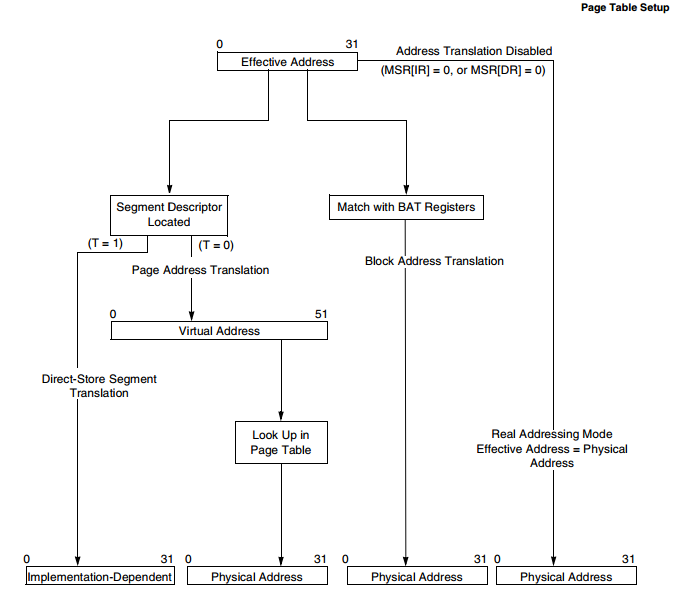
\includegraphics[scale=0.5]{PPC_addressing_flow}
   \caption{PowerPC Address Translation Modes}
\end{figure}
\par

Block Address Translation allows for virtual memory to be directly mapped to real, contiguous memory addresses. Being able to map data structures directly into virtual memory is important for applications that require heavy disk IO. The translation is mapped by 8 pairs of registers, 4 each for data and instructions, each mapping to 128KB or larger contiguous blocks of memory. BAT is always performed first when looking up physical addresses. If translation with BAT succeeds then the page table translation stops.  If BAT fails then the EA is translated by looking up the page table in Segmented Address Translation mode. 
\par
Pages in PowerPC can cover up to 4KB of memory for an 8 byte entry, with a maximum addressable space of 4GB in 32 bit systems, and 256 TB in 64 bit systems. PPC uses a hashed page table that exists in main for fast lookup (hash tables have a constant time lookup fee) between virtual and real page numbers. For each EA there are 23 or 52 bits reserved for the Virtual Segment ID (VSID). The VSID is  logical ORd with the first four bits of the EA to get the virtual address (VA). The VA is then hashed to identify the Page Table Entry Group (PTEG). The Page Table Entries (PTE) are then each tested for a valid real address. If it is found then the lookup returns, otherwise there is a secondary hash computed out of the VSID and the EA. The PTEGs and PTEs are then tested for the real address, if it is not found here, then a page found exception is raised. SAT lookups are done in parallel with BAT lookups, and BAT will be used in favor of SAT if it succeeds. 

\par
\begin{figure}[h]
   \centering
   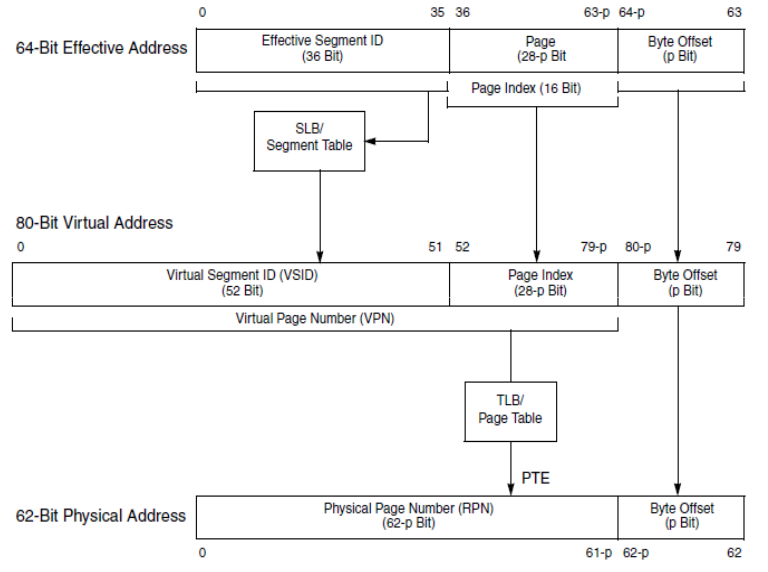
\includegraphics[scale=0.5]{PPC_address}
   \caption{Segmented Address Translation}
\end{figure}
\par

The paging structure of Intel's 64 bit x86 systems can be modeled as a hierarchy as well. Paging on IA exists as a memory management system designed to control memory access in main memory. The entire addressable main memory space is divided into pages with a read address mappable to a 48 bit addressing space. This space is broken up into pages and tables with their respective directories. The PA is calculated based on the contents of the linear address given. Different bits in the linear address correspond to offsets (locations) in the directory tree structure, eventually leading to the physical address. The way the bits are arranged depends on the paging mode that the processor is in. IA32e paging is one of three paging modes supported by the x86 architecture. IA32e translates the 48 bit linear addresses to a 52 bit physical address. The IA32e mode does the first look up in the CR3 control register to find the first paging structure location, the PML4. The bit alignment in the CR3 register depends on if CR4.PCIDE is set. The logical processor determines the type of memory to be used to access the address based on the values in CR3.PWD and CR3.PCD. IA32e may map addresses with 4KB, 2MB, or 1GB page size, much larger than any PPC page. There are proportionately fewer pages when the size is extended to 1GB. The page directory is found using the values held in PDTPE 51:30. The system then navigates to the directory in PDE and then to the physical address. Each physical address also comes with a protection key, which determines access rights to the physical address. The processor may speed up the translation of addresses by caching addresses in a TLB. The TLB entry will contain an individual translation that has been used recently. 

\par
\begin{figure}[h]
   \centering
   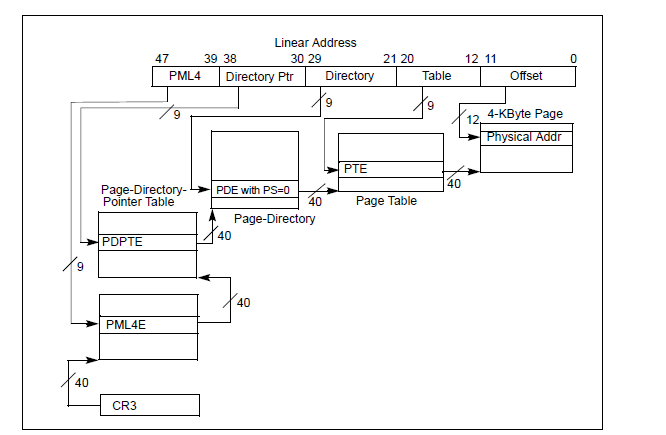
\includegraphics[scale=0.5]{IA_paging}
   \caption{x86 Address Translation}
\end{figure}
\par

\section{High Performance Computing}

\textsc{There} is a variant of the PPC 750 that is radiation-hardened and used for military and aerospace applications. The RAD750 is manufactured by BAE Systems Electronics, and launched the first unit into space in 2005. The RAD750 is made using 150 nm lithography, much smaller than the PPC 750 which was first manufactured at over 200 nm. Over 150 RAD750 boards have been launched into space, and each board costs on the order of 200,000 USD. 
\par
Intel is the standard when it comes to high performance computing. Xeon processors are multi-core up to 18 cores and boast huge throughput. Many of the fastest supercomputers in the world have been made with Intel inside. Intel`s Xeon Phi line offers massively parallel systems, up to 72 cores in the new Knight’s Landing line of Xeon Phi boards. Years of building upon vectorized instructions, SSE, MMX, and a hardware intensive pipeline have made Intel a powerhouse for throughput. PPC is much older and does not support SIMD instructions, much less anything like MMX. 
\par

\section{Conclusion}

\textsc{Comparing} PPC and IA is in some ways is extremely unfair, the PPC 750 is far older than any modern 18 core Xeon card, and can\’t possibly have the same capabilities. But Intel started far behind IBM when they first launched their 8086, IBM was the industry standard for processors. Intel now dominates the market, most likely bordering on an illegal level of command over the processor industry. But the PPC and IA are very different architectures no matter how they`re compared. PPC offers 32 GPRs, far more than IA. PPC also offers a simpler instruction set that could still be more useful in smaller applications when a powerhouse x86 is too much (discounting the possibility of ARM for the sake of argument). PPC offers a simpler memory model, and the details of the architecture are far more exposed than Intel`s architectures, which may matter so some engineers and architects. The PowerPC is a tribute to time’s wearing as it was birthed from a powerful alliance, but was eventually superseded by the then smaller x86. 
\par 
\pagebreak

\clearpage
\section{Bibliography}
    \begin{itemize}
        \item[1:] Wikipedia, 'IBM POWER Instruction Set Architecture', 2015. [Online]. Available: https://en.wikipedia.org/wiki/IBM\_POWER\_Instruction\_Set\_Architecture. [Accessed: 08- Dec- 2015].
        \item[2:] PowerPC™ Microprocessor Family: The Programming Environments For 32-Bit Microprocessors, 1st ed. 2015.
        \item[3:] PowerPC 750 Microprocessors, 1st ed. 2015.
        \item[4:] Single Board Computer for Space, 1st ed. 2015.
        \item[5:] C. Wai, Comparative study of the Pentium and PowerPC family of micro-processors, 1st ed. 2015.
        \item[6:] The PowerPC Compiler Writer’s Guide, 1st ed. 2015.
        \item[7:] Intel® ARK (Product Specs), 'ARK | Compare Intel® Products', 2015. [Online]. Available: http://ark.intel.com/compare/84679,84678,84677,84676,84688,84686,84685. [Accessed: 08- Dec- 2015]. 
        \item[8:] S. McFarling Combining Branch Predictors Digital Western Research Lab (WRL) Technical Report, TN-36, 1993:8
    \end{itemize}


\end{document}
